\documentclass[11pt]{article}
\usepackage{amsmath,amssymb,epsfig,graphics,hyperref}

\hypersetup{colorlinks=true}

\setlength{\textwidth}{7in}
\setlength{\topmargin}{-0.575in}
\setlength{\textheight}{9.25in}
\setlength{\oddsidemargin}{-.25in}
\setlength{\evensidemargin}{-.25in}

\title{\bf Notes about problems from a variety of sources}
\author{\bf Shuo Yang}

\begin{document}

\maketitle

\begin{center}
Last updated: \date{\today}
\end{center}

\section*{\bf Stanford-cs103 spring14 hw5}

\emph{Problem 1b}

After playing around with some examples, I found that a string is
accepted in one of the following cases.

\begin{enumerate}
\item $\epsilon$
\item $a^+$
\item $b^+$
\item $ba$
\item $(ab^+aa)(a^*baa)^*$
\item $(baa^+b)(b^*aa^+b)^*a?$
\end{enumerate}


So the regular expression for the language should be the union of the
above cases.

Note that strings with consecutive $ab's$ can never be accepted.

below is the DFA I built:\\

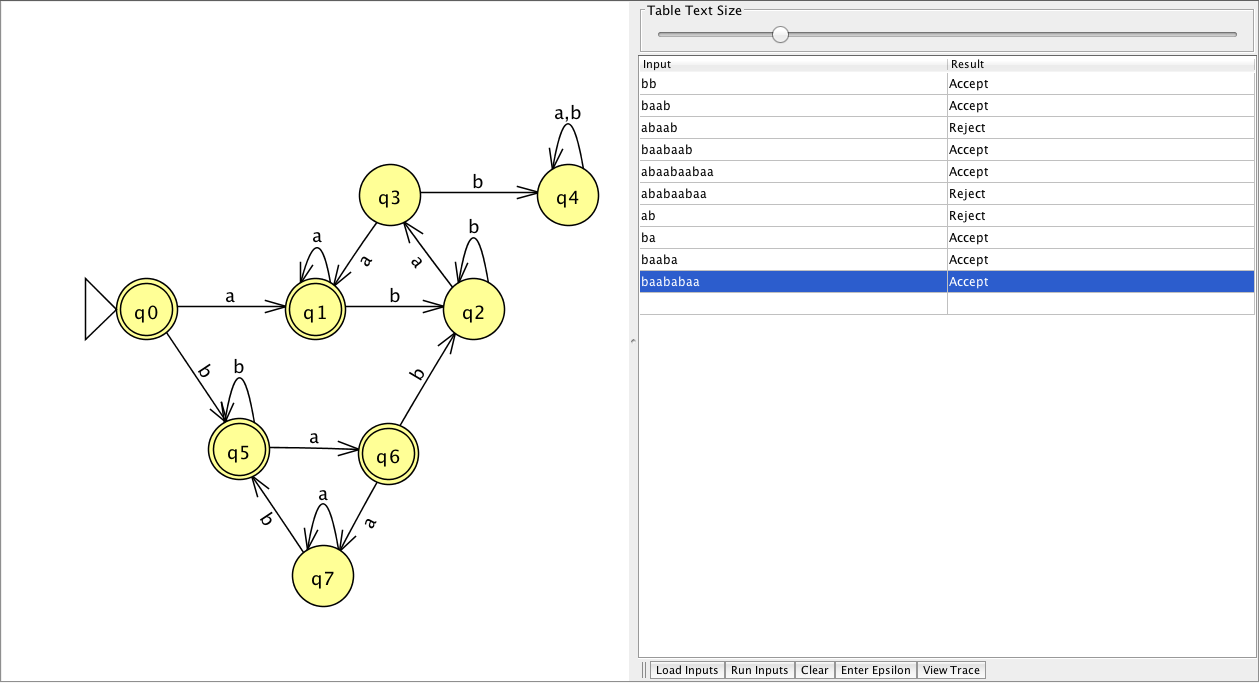
\includegraphics[width=15cm,height=8cm]{../imgs/dfa-stanford-cs103-spring14-hw5-1b.png}
\end{document}
